\documentclass[a4paper,12pt]{report}
\usepackage{graphicx}
\graphicspath{{picaa/}}
\usepackage{listings}
\usepackage{amsmath}
\usepackage[T2A]{fontenc}
\usepackage[utf8]{inputenc}
\usepackage[english,russian]{babel}
\usepackage{pgfplots} 
\usepackage{indentfirst}
\parindent=1cm

\usepackage{geometry}
\geometry{left=2cm}
\geometry{right=1.5cm}
\geometry{top=1cm}
\geometry{bottom=2cm}
\lstset{language = C++,
	keywordstyle = \color{orange},
	commentstyle = \color{red},
	columns = fullflexible
}

\begin{document}

    \begin{titlepage}

        \begin{center}
            \large
            \textbf{Государственное образовательное учреждение высшего профессионального образования\\
            “Московский государственный технический университет имени Н.Э.Баумана”\\}
            
\includegraphics{bmstu-logo.png}
			\vspace{1cm}
            
            \textsc{Дисциплина: Анализ алгоритмов}
            \vspace{0.5cm}
                
            \textsc{Лабораторная работа №5}
            \vspace{1cm}
            
            {\LARGE \textbf{Конвейер}}
            \vspace{3cm}
                    
            \begin{flushright}
            	Студент группы ИУ7-55Б,\\   
            	Руднев К. К.,\\
            	\vspace{0.5cm}
            	Преподаватель,\\
            	Волкова Л. Л.,\\
            	Строганов Ю. В.
            	
            \end{flushright}
            \vfill
            
            2019 г.
            
            \end{center}

    \end{titlepage}

	\setcounter{page}{2}
	\tableofcontents
    \chapter*{Введение}

        	Выполнение каждой команды складывается из ряда последовательных этапов (шагов, стадий), которые не меняются от команды к команде. 
        	С целью увеличения быстродействия процессора и максимального использования всех его возможностей в современных микропроцессорах используется конвейерный принцип обработки информации. Этот принцип подразумевает, что в каждый момент времени процессор работает над различными стадиями выполнения нескольких команд, причем на выполнение каждой стадии выделяются отдельные аппаратные ресурсы. По очередному тактовому импульсу каждая команда в конвейере продвигается на следующую стадию обработки, выполненная команда покидает конвейер, а новая поступает в него.
        	
        	Конвейерная обработка в общем случае основана на разделении подлежащей исполнению функции на более мелкие части и выделении для каждой из них отдельного блока аппаратуры. Производительность при этом возрастает благодаря тому, что одновременно на различных ступенях конвейера выполняются несколько команд. Конвейерная обработка такого рода широко применяется во всех современных быстродействующих процессорах.
        	
        	\vspace{0.5cm}
			Цель работы: получить навык организации асинхронной передачи данных между потоками на примере конвейерной обработки информации.\\
			
			Задачи работы:\\
			\begin{enumerate} 
				\item выбрать и описать методы обработки данных, которые будут сопоставлены методам конвейера;\\
				\item описать архитектуру программы, а именно какие функции имеет главный поток, принципы и алгоритмы обмена данными между потоками;\\
				\item реализовать конвейерную систему, а также сформировать лог событий с указанием времени их происхождения, описать реализацию;\\
				\item провести тестирование системы.\\
			\end{enumerate}
        \label{sec:intro}

    \newpage

    \chapter{Аналитическая часть}
    
        \label{sec:analitic_part}
        	В рамках раздела будет дано аналитическое описание конвейерной системы обработки. Также будет определено, что должно обрабатываться такой системой.
	
	\section{Общие сведения о конвейерной  обработке}

			\textbf{Конвейер} – машина непрерывного транспорта \cite{mednov}, предназначенная для перемещения сыпучих, кусковых или штучных грузов.

			\textbf{Конвейерное производство} - система поточной организации производства на основе конвейера, при которой оно разделено на простейшие короткие операции, а перемещение деталей осуществляется автоматически. 
			Это такая организация выполнения операций над объектами, при которой весь процесс воздействия разделяется на последовательность стадий с целью повышения производительности путём одновременного независимого выполнения операций над несколькими объектами, проходящими различные стадии. 
			Конвейером также называют средство продвижения объектов между стадиями при такой организации\cite{wiki}. 
			Появилось в 1914 году на производстве Модели-Т на заводе Генри Форда\cite{ford} и произвело революцию сначала в автомобилестроении, а потом и в промышленности в целом.
		
	\section{Описание алгоритмов}
        
			В данной лабораторной работе реализована некая функцию хеширования строки, которая состоит из трех последовательных действий: применения первой хеш-функции, применения второй хеш-функции и применения третьей хеш-функции. 
			Если необходимо вычислить хеш для какого-то массива строк, то можно использовать конвейерную обработку данных. 
			Таким образом задача будет решена эффективнее, чем при последовательном применении алгоритмов к массиву значений.  
			Конвейер будет состоять из четырех уровней. 
			Обработанные данные передаются последовательно с одного уровня (одной ленты) конвейера на следующий (следующую ленту). 
			Далее на каждом уровне осуществляется обработка данных, занимающая определенное время. 
			Для каждой ленты создается своя очередь задач, в которой хранятся все необработанные строки. 
			На последнем уровне конвейера обработанные объекты попадают в пул обработанных задач.
			
			\vspace{0.5cm}
			Уровни конвейера:
			\begin{itemize}
				\item 0 уровень — генерация входных данных в первую очередь;
				\item 1 уровень (лента) — применение первого хеша к строкам из первой очереди, задержка + задержка 1с, запись результата во 2 очередь;
				\item 2 уровень (лента) — применение второго хеша к строкам 2 очереди + задержка 3с, запись результата в 3 очередь;
				\item 3 уровень (лента) — применение третьего хеша к строкам 3 очереди + задержка 1,5с, запись результата в пул обработанных задач.
			\end{itemize}
		
			Поскольку запись в очередь и извлечение из очереди это не атомарные операции, необходимо создать их таковыми путем использования мьютексов (по одному на одну очередь) и критических секций, чтобы избежать ошибок в ситуации гонок.
			
	\section{Вывод}

			В данном разделе была рассмотрена идея конвейерной обработки, а также была описана схема конвейерной обработки, используемой для реализации в лабораторной работе.

    \newpage

    \chapter{Конструкторская часть}
        \label{sec:construct_part}
        
			В дальнейшем на рисунках \ref{ris:conv1}-\ref{ris:conv3}  будут представлены схемы расматриваемого алгоритма.
			Рисунок \ref{ris:conv1} изображает схему работы конвейерной обработки данных.
			Рисунок \ref{ris:conv2} изображает схему работы главного потока. 
			Рисунок \ref{ris:conv3} изображает схему работы ленты конвейера.

	\section{Разработка алгоритмов}

		\begin{figure}[h!]
			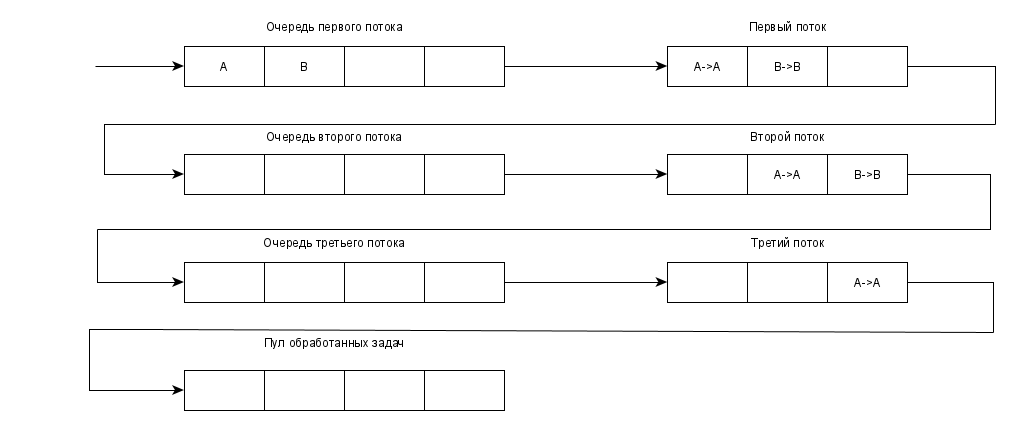
\includegraphics[width=1\linewidth]{conveyor1.png}
			\caption{Схема конвейерной обработки}
			\label{ris:conv1}
		\end{figure}
	
		\newpage
	
		\begin{figure}[h!]
			\center{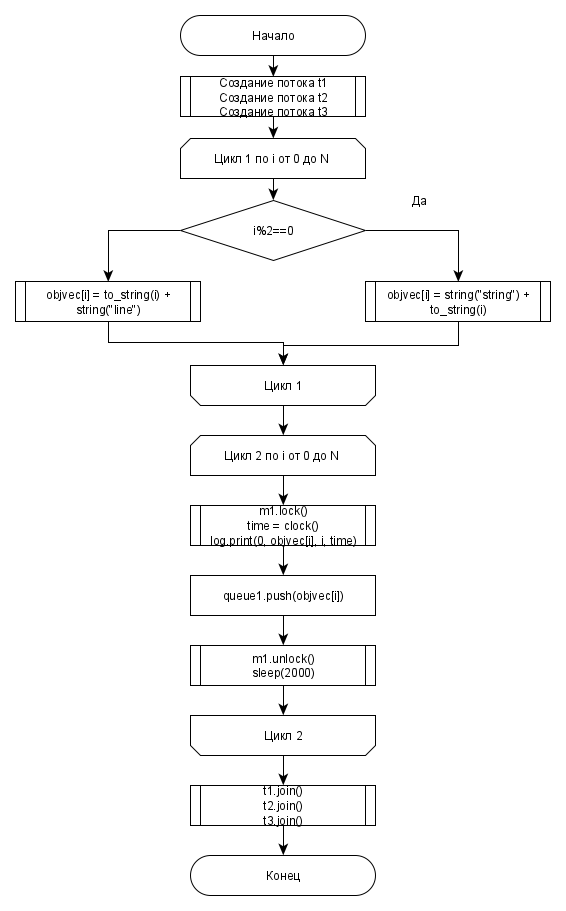
\includegraphics[width=0.8\linewidth]{con11.png}}
			\caption{Схема главного потока}
			\label{ris:conv2}
		\end{figure}
	
		\newpage
	
		\begin{figure}[h!]
			\center{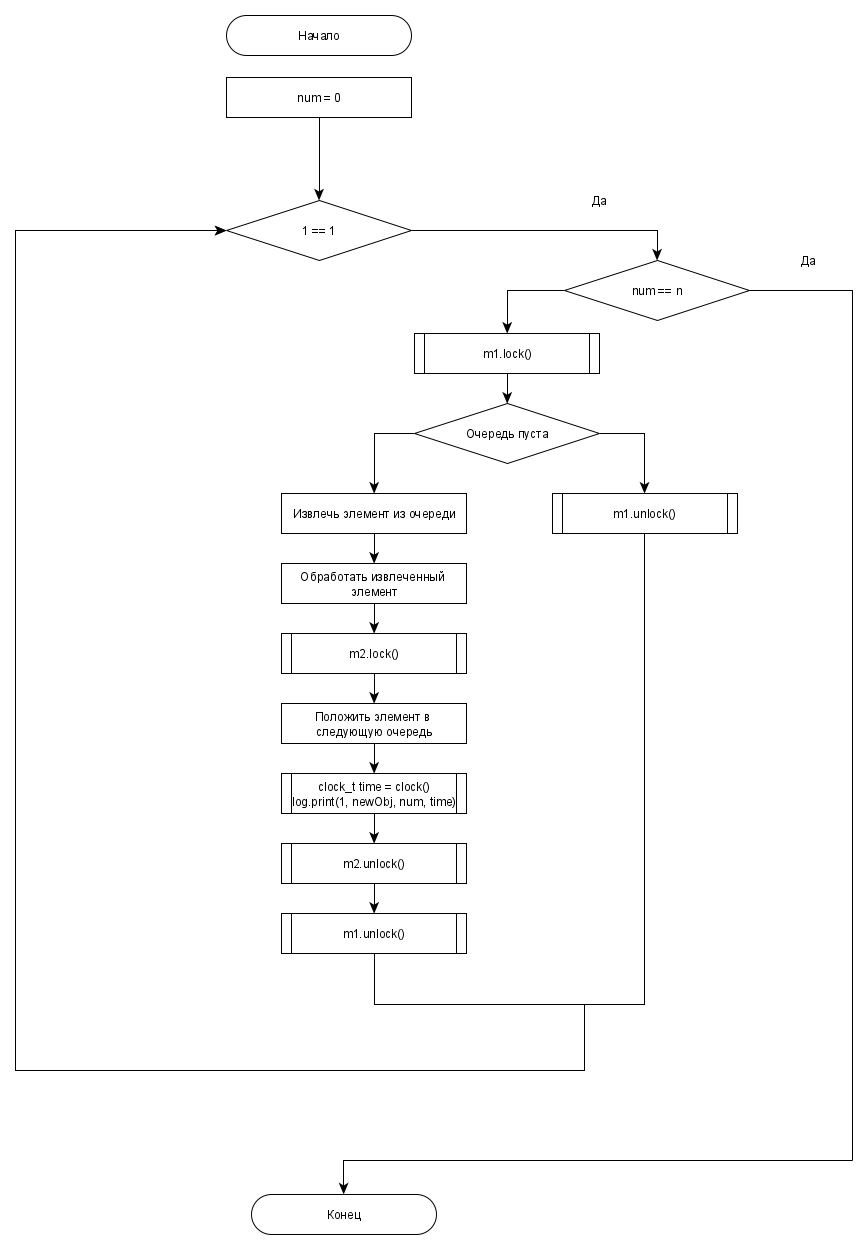
\includegraphics[width=1\linewidth]{con21.png}}
			\caption{Схема рабочего потока}
			\label{ris:conv3}
		\end{figure}

    \newpage
    
    \section{Вывод}
    
    В рамках раздела были рассмотрены схемы конвейерной обработки данных с целью их дальнейшего переноса в программу.
    
    \newpage

    \chapter{Технологическая часть}
    
        \label{sec:tecnologic_part}
			В рамках раздела будут описаны инструментарии разработки, выбор среды, требования к ПО. 
			Также будут предоставлены листинги конкретных реализаций алгоритмов.
			
			Замеры времени были произведены на: Intel(R) Core(TM) i7-8565U, 4 ядра, 8 логических процессоров.
	
	\section{Средства реализации}	
			
			Для реализации алгоритмов использовался язык программирования C++ 17 и среда разработки QtCreator Community Edition 5.5. 
        	У данного языка имеются удобные библиотеки для написания мультипоточных приложений, чего будет достаточно для реализации текущей лабораторной работы, а среда разработки имеет бесплатную коммьюнити версию и подходящий компилятор, позволяющий использовать std::threads.
        	
        	Замер времени реализован с помощью функции clock() из библиотеки time.h.
        	Измеряется время исполнения кода чистого алгоритма (без учета времени на создание потоков, очередей, генерацию данных и т.п.).

	\section{Требования к программному обеспечению}

			На вход программа должна получать набор данных - в данной программе это набор строк для хеширования. 
			
			На выход программа должна выдавать захешированную строку по заранее определенным хеш-функциям. 
			Дополнительно выводятся временные метки для наблюдения за работой конвейерного типа обработки данных.

	\section{Листинг кода}
	
        	На листингах \ref{list:help}-\ref{list:main} представлена реализация конвейерной обработки данных.
	        На листинге \ref{list:help} представлен код вспомогательных классов и объявлений.
	        На листингах \ref{list:first}-\ref{list:third} представлен код конвейерных лент.
	        На листинге \ref{list:main} представлен код управляющей функции программы.
	        
	        \begin{lstlisting}[frame = single, label = list:help, breaklines, caption = Вспомогательные классы и объявления]
	#include <iostream>
	#include <queue>
	#include <thread>
	#include <vector>
	#include <mutex>
	#include <stdlib.h>
	#include <unistd.h>
	#include <ctime>
	        
	using namespace std;
	typedef string input_t;
	        
	static queue<input_t> queue1;
	static queue<input_t> queue2;
	static queue<input_t> queue3;
	        
	static vector<input_t> objvec;
	static vector<input_t> res;
	        
	static mutex m1, m2, m3, resm;
	static int n = 10;
	        
	FILE *f;
	static clock_t main_time = clock();
	static clock_t mtime = clock();
	        
	class Logger
	{
	public:
	    Logger() {}
	    static void print(int step, string str, int i, clock_t time = 0)
	    {
	    	fprintf(f,"[%d] step item%d time: %ld (%ld)  value: %s\n", step, i, time, time - mtime, str.c_str());
	        std::cout << step <<" step: "<< "  item" << i << " " << " time: "<< time - main_time<<"  " << str  << std::endl;
	        mtime += time - mtime;
	    }
	};
	Logger log; 
	        \end{lstlisting}
	        
	        \begin{lstlisting}[frame = single, breaklines, label = list:first, caption = Первая конвейерная лента]
	void SingleHash()
	{
	    int num = 0;
	    while (1)
	    {
	        if (num == n)
	            break;
	        
	        m1.lock();
	        if (queue1.empty())
	        {
	            m1.unlock();
	            continue;
	        }
	        
	        input_t myObj = queue1.front();
	        queue1.pop();
	        m1.unlock();
	        
	        input_t newObj = myHash1(myObj);
	        m2.lock();
	        queue2.push(newObj);
	        sleep(1);
	        clock_t time = clock();
	        log.print(1, newObj, num, time);
	        m2.unlock();
	        
	        num++;
	    }
	}
	        \end{lstlisting}
	        	
	        \begin{lstlisting}[frame = single, breaklines, label = list:second, caption = Вторая конвейерная лента]
	void MultiHash()
	{
	    int num = 0;
	    while (1)
	    {
	        if (num == n)
	            break;
	        
	        m2.lock();
	        if (queue2.empty())
	        {
	            m2.unlock();
	            continue;
	        }
	        
	        input_t myObj = queue2.front();
	        queue2.pop();
	        m2.unlock();
	        
	        input_t newObj = myHash2(myObj);
	        m3.lock();
	        queue3.push(newObj);
	        sleep(3);
	        clock_t time = clock();
	        log.print(2, newObj, num, time);
	        m3.unlock();
	        
	        num++;
	    }
	}
	        \end{lstlisting}
	
	        \begin{lstlisting}[frame = single, breaklines, label = list:third, caption = Третья конвейерная лента]
	void Result()
	{
	    int num = 0;
	    while (1)
	    {
	        if (num == n)
	            break;
	        
	        m3.lock();
	        if (queue3.empty())
	        {
	            m3.unlock();
	            continue;
	        }
	        
	        input_t myObj = queue3.front();
	        queue3.pop();
	        m3.unlock();
	        input_t newObj = myHash3(myObj);
	        resm.lock();
	        
	        res.push_back(newObj);
	        sleep(1.5);
	        clock_t time = clock();
	        log.print(3, newObj, num, time);
	        resm.unlock();   
	        num++;
	    }
	}
	        \end{lstlisting}
	        
	        \begin{lstlisting}[frame = single, breaklines, label = list:main, caption = Основная функция программы]
	int main()
	{
	    f = fopen("res.txt", "w");
	    n = 10;
	    objvec.resize(n);
	        
	    thread t1(SingleHash);
	    thread t2(MultiHash);
	    thread t3(Result);
	    main_time = clock();
	    for (int i = 0; i < n; i++)
	    {
	        if (i % 2 == 0)
	        {
	            objvec[i] = string("string") + to_string(i);
	        }
	        else
	        {
	            objvec[i] = to_string(i) + string("line");
	        }
	    }
	        
	    for (int i = 0; i < n; ++i)
	    {
	        clock_t time = clock();
	        log.print(0, objvec[i], i, time);
	        m1.lock();
	        
	        queue1.push(objvec[i]);
	        m1.unlock();
	        sleep(2);
	    }
	        
	    if (t1.joinable())
	        t1.join();
	    if (t2.joinable())
	        t2.join();
	    if (t3.joinable())
	        t3.join();
	    fclose(f);
	    return 0;
	}
	        \end{lstlisting}

	\section{Вывод}
	
	В рамках раздела были предъявлены требования к программному обеспечению. 
	На основании их были разработана и представлена конкретная реализация конвейерной обработки данных.

    \newpage

    \chapter{Экспериментальная часть}
        \label{sec:experimental_part}

			В рамках раздела будут предоставлены тесты программы, представленные на листинге \ref{list:test}. 
			Будут проведены эксперименты по вычислению времени выполнения рассматриваемого алгоритма.

	\section{Примеры работы}

        	На листинге \ref{list:test} представлена структура файла-результата. 
        	Для упрощения отслеживания работы конвейера были добавлены временные метки, а также промежуточные результаты, показывающие, какая лента совершила те или иные действия с объектом.

		\begin{lstlisting}[frame = single, label=list:test, caption= Файл с результатом]
[0]  item0 time: 9 (0)  value: string0
[1]  item0 time: 1019 (1010)  value: DFE=C=W~DGG@GB]
[0]  item1 time: 2018 (999)  value: 1line
[2]  item0 time: 4027 (2009)  value: jki`e^'Mbdc[a[%_ehhahc.Vm!"l$p<~eijdlh4]%*,'0J_[^^
W^Y$Lcghbjf2
[1]  item1 time: 5037 (1010)  value: R><B:~R?>E>
[0]  item2 time: 5037 (0)  value: string2
[3]  item0 time: 5537 (500)  value: resultJKI@E>W-BDC;A;U?EHHAHC^6MQRLTPl^EIJDLH
d=UZ\W`]*?;>>7>9T,CGHBJFbhash
[2]  item1 time: 8545 (3008)  value: (c`e\O"^\bZ_#`_f_T)ggoi~#aaicY/no(#_iVU\UJo]]e_
[1]  item2 time: 9555 (1010)  value: DFE=C=Y~DGG@GB_
[0]  item3 time: 9555 (0)  value: 3line
[3]  item1 time: 10054 (499)  value: resultXC@E</R><B:?S@?F?4YGGOI^SAAIC9_NOXS
?I65<5*O==E?hash
[2]  item2 time: 13063 (3009)  value: jki`e^)Mbdc[a['_ehhahc0Vm!"l$p>~eijdlh6]%*,'0-L_
[^^W^Y&Lcghbjf4
[1]  item3 time: 14072 (1009)  value: T><B:~T?>E>
[0]  item4 time: 14072 (0)  value: string4
[3]  item2 time: 14572 (500)  value: resultJKI@E>Y-BDC;A;W?EHHAHC`6MQRLTPn^
EIJDLHf=UZ\W`],?;>>7>9V,CGHBJFdhash
[2]  item3 time: 17580 (3008)  value: *c`e\O$^\bZ_%`_f_T+ggoi~%aaicY1no(#_kVU\
UJ!]]e_
[1]  item4 time: 18590 (1010)  value: DFE=C=[~DGG@GBa
[3]  item3 time: 19090 (500)  value: resultZC@E</T><B:?U@?F?4[GGOI^UAAIC9aNOXS
?K65<5*Q==E?hash
[2]  item4 time: 22108 (3018)  value: jki`e^+Mbdc[a[)_ehhahc2Vm!"l$p@~eijdlh8]%*,'0-N_
[^^W^Y(Lcghbjf6
[3]  item4 time: 23617 (1509)  value: resultJKI@E>[-BDC;A;Y?EHHAHCb6MQRLTPp^EIJD
LHh=UZ\W`].?;>>7>9X,CGHBJFfhash
		\end{lstlisting}
		
			Лог файл состоит из записей отсортированных по времени с начала запуска приложения. 
			В первом столбце указан номер лининии обработки, затем номер текущего элемента, затем время с начала работы программы и время выполнения данного этапа в миллисекундах, а также значение хеша на текущем этапе.
			
			По листингу можно проследить выполнение каждого этапа  и изменение значений хеша при обработке на каждой из лент. 
			Также можно проследить, что обработка выполняется параллельно. 
			Например, 2 линия не ждет полного завершения работы первой прежде, чем начать работу, а начинает выполнение как только в очередь поступает новый элемент. 
			Так как обработка на каждой линии занимает разное количество времени, в листинге можно увидеть, насколько она эффективнее.
			При последовательной обработке каждого элемента потребовалось бы $$(1000 + 3000 + 1500) * 5 = 27500ms.$$ 
			Но алгоритм завершился за 23617ms, что приносит выигрыш в 4s.
        
    \section{Вывод}

        Алгоритм конвейерной обработки эффективен для ситуаций, когда каждая линия конвейера требует разное время на обработку задачи. 
        Однако в случае, когда  все линии обрабатывают задачи за одинаковое время, алгоритм не будет давать существенного выигрыша. 
        В рамках лабораторной работы с примитивными задачами конвейер принес 15\% выигрыш по времени выполнения.

    \newpage

    \chapter*{Заключение}
        \label{sec:conclusion_part}
        
        В результате выполнения данной работы рассмотрено и изучено понятие конвейерной обработки данных. 
        Реализован простейший конвейер на три линии. Сравнены временные характеристики при конвейерной и последовательной обработке данных. 
        
        В ходе экспериментов оказалось, что даже для самых приитивных задач конвейерная обработка позволяет сэкономить 15\% времени работы.
        
     \begin{thebibliography}{3}
    	\bibitem{mednov} Меднов В.П., Бондаренко Е.П. Транспортные, распределительные и рабочие конвейеры. М., 1970.
    	\bibitem{wiki} Конвейерное производство[Электронный ресурс] - режим доступа https:/dic.academic.ru/dic.nsf/ruwiki/1526795
    	\bibitem{ford} Koнвeйepный meтoд пpoизвoдcтвa Гeнpи Фopдa[Электронный ресурс] - режим доступа https://popecon.ru/305-konveiernyi-metod-proizvodstva-genri-forda.html
    	\bibitem{Beloysov} И. В. Белоусов(2006), Матрицы и определители, учебное пособие по линейной алгебре, с. 1 - 16
    	\bibitem{Gall2012}
    	Le Gall, F. (2012), "Faster algorithms for rectangular matrix multiplication", Proceedings of the 53rd Annual IEEE Symposium on Foundations of Computer Science (FOCS 2012), pp. 514–523
    \end{thebibliography}
\end{document}
